\chapter{Teorii și tehnologii utilizate}

În acest capitol sunt prezentate în primul rând tehnologiile utilizate în implementarea aplicației. În cea de a doua parte este evidențiat în mare parte particularități ale algoritmicii utilizate în determinarea unei alocări optime specifice problemei, în alte cuvinte algoritmul de \textit{stable matching} (\textit{stable marriage}).

\section{Angular}
\begin{figure}[H]
	
\includegraphics[width=0.3\textwidth, left]{Angular-logo.png}
%	\caption{\url{https://www.vectorlogo.zone/logos/angular/angular-ar21.png}}
\end{figure}

\textbf{Angular} este un framework de JavaScript scris în TypeScript și menținut de Google. Framework-ul a fost dezvoltat în principal pentru crearea aplicațiilor web \textit{single-page}, într-o manieră ce ușurează mentenanța și dezvoltarea ulterioară.

\subsection{Scurt istoric}
În 2010, Miško Hevery, un angajat la Google la acel timp, a lansat un proiect cu numele \textit{AngularJS} care a fost apreciat în mare măsură de comunitate. Între anii 2014-2015 a avut loc o reîmprospăatare majoră a framework-ului însemnând de fapt o rescriere majoră a acestuia. Noua versiune avea să fie numită simplu Angular. Au urmat câțiva ani de tranziție deoarece multe proiecte deja în producție erau utilizau AngularJS și  trebuiau refactorizate. În acest moment, Angular este cel mai folosit framework de front-end, în specialde dezvoltatorii de la Google și de către start-up-uri. Exemple de companii recunoscute ce folosesc Angular sunt Microsoft, Gmail, PayPal, Forbes.

\begin{figure}[H]
	\centering
	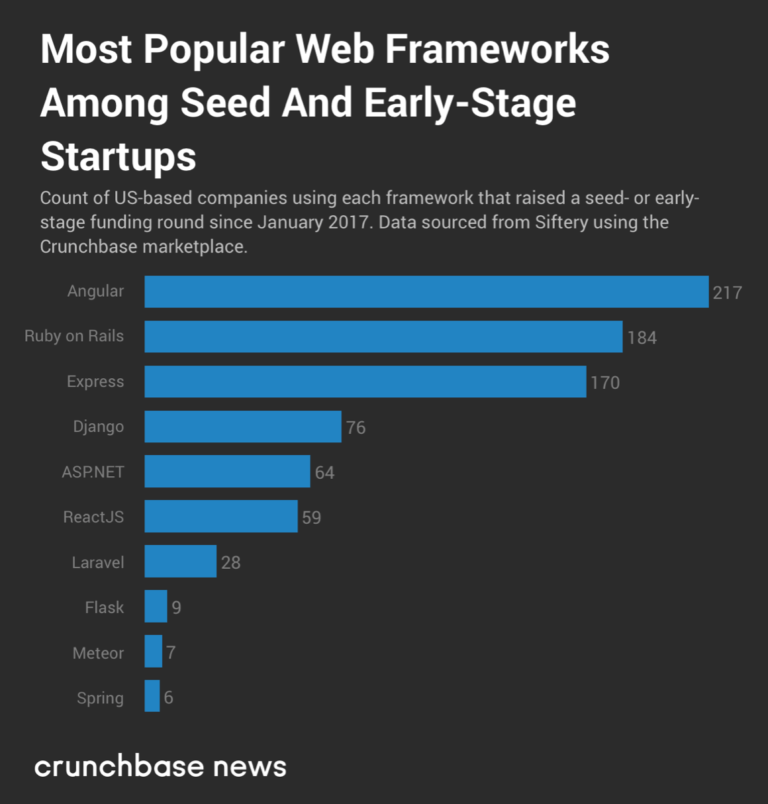
\includegraphics[width=0.8\textwidth]{Angular-crunchbase-newspng.png}
	\caption{\url{https://www.moveoapps.com/blog/how-to-use-angular-development/}}
\end{figure}

\subsection{Particularități}
Motivul alegerii Angular pe partea de front-end este reprezentat de o serie de caracteristici.

Un astfel de motiv este \textit{arhitectura bazată pe componenta}, fiind astfel o formă de programare orientată pe obiect. Utilizatorul crează în mod uzual clase corespunzătoare componentelor ce conțin și un șablon HTML (\textit{eng.} HTML template). Pentru simplificare, Angular oferă și opțiunea de "injectare" a serviciilor \textit{custom} sau \textit{in-built} într-o componentă ce utilizează aceste funcționalități. În acest fel, utilizatorul poate reutiliza, înlocui, modifica componente în diverse locuri, obținâându-se astfel un UI (User Interface) modularizat.

Un alt motiv este modul de încărcare a paginii web. Angular folosește \textit{lazy loading} ce permite încărcarea instantanee a website-urilor, prin afișarea doar a componentelor cerute și necesare utilizatorului, în timp ce celelalte sunt pregătite în fundal pentru alte eventualități.

\textit{Dependency injection} reprezintă un al treilea motiv, un design pattern ce permite împărțirea lucrului între diferite servicii, distribuind în mod eficient sarcinile. Prin inițializarea dependențelor, Angular reușește să reducă în mod considerabil codul de tip \textit{boilerplate} (fragmente similare de cod des utilizat între care există mici diferențe) și să extindă mai ușor o astfel de aplicație.

Framework-ul are trei tipuri de \textit{dependency injections}:
\begin{enumerate}
	\item Constructor injection
	\item Setter injection
	\item Interface injection
\end{enumerate}

Din punct de vedere al arhitecturii, Angular este în totalitate un framework MVC (model-view-controller), după cum se observă în figura următoare.

\begin{figure}[H]
	\centering
	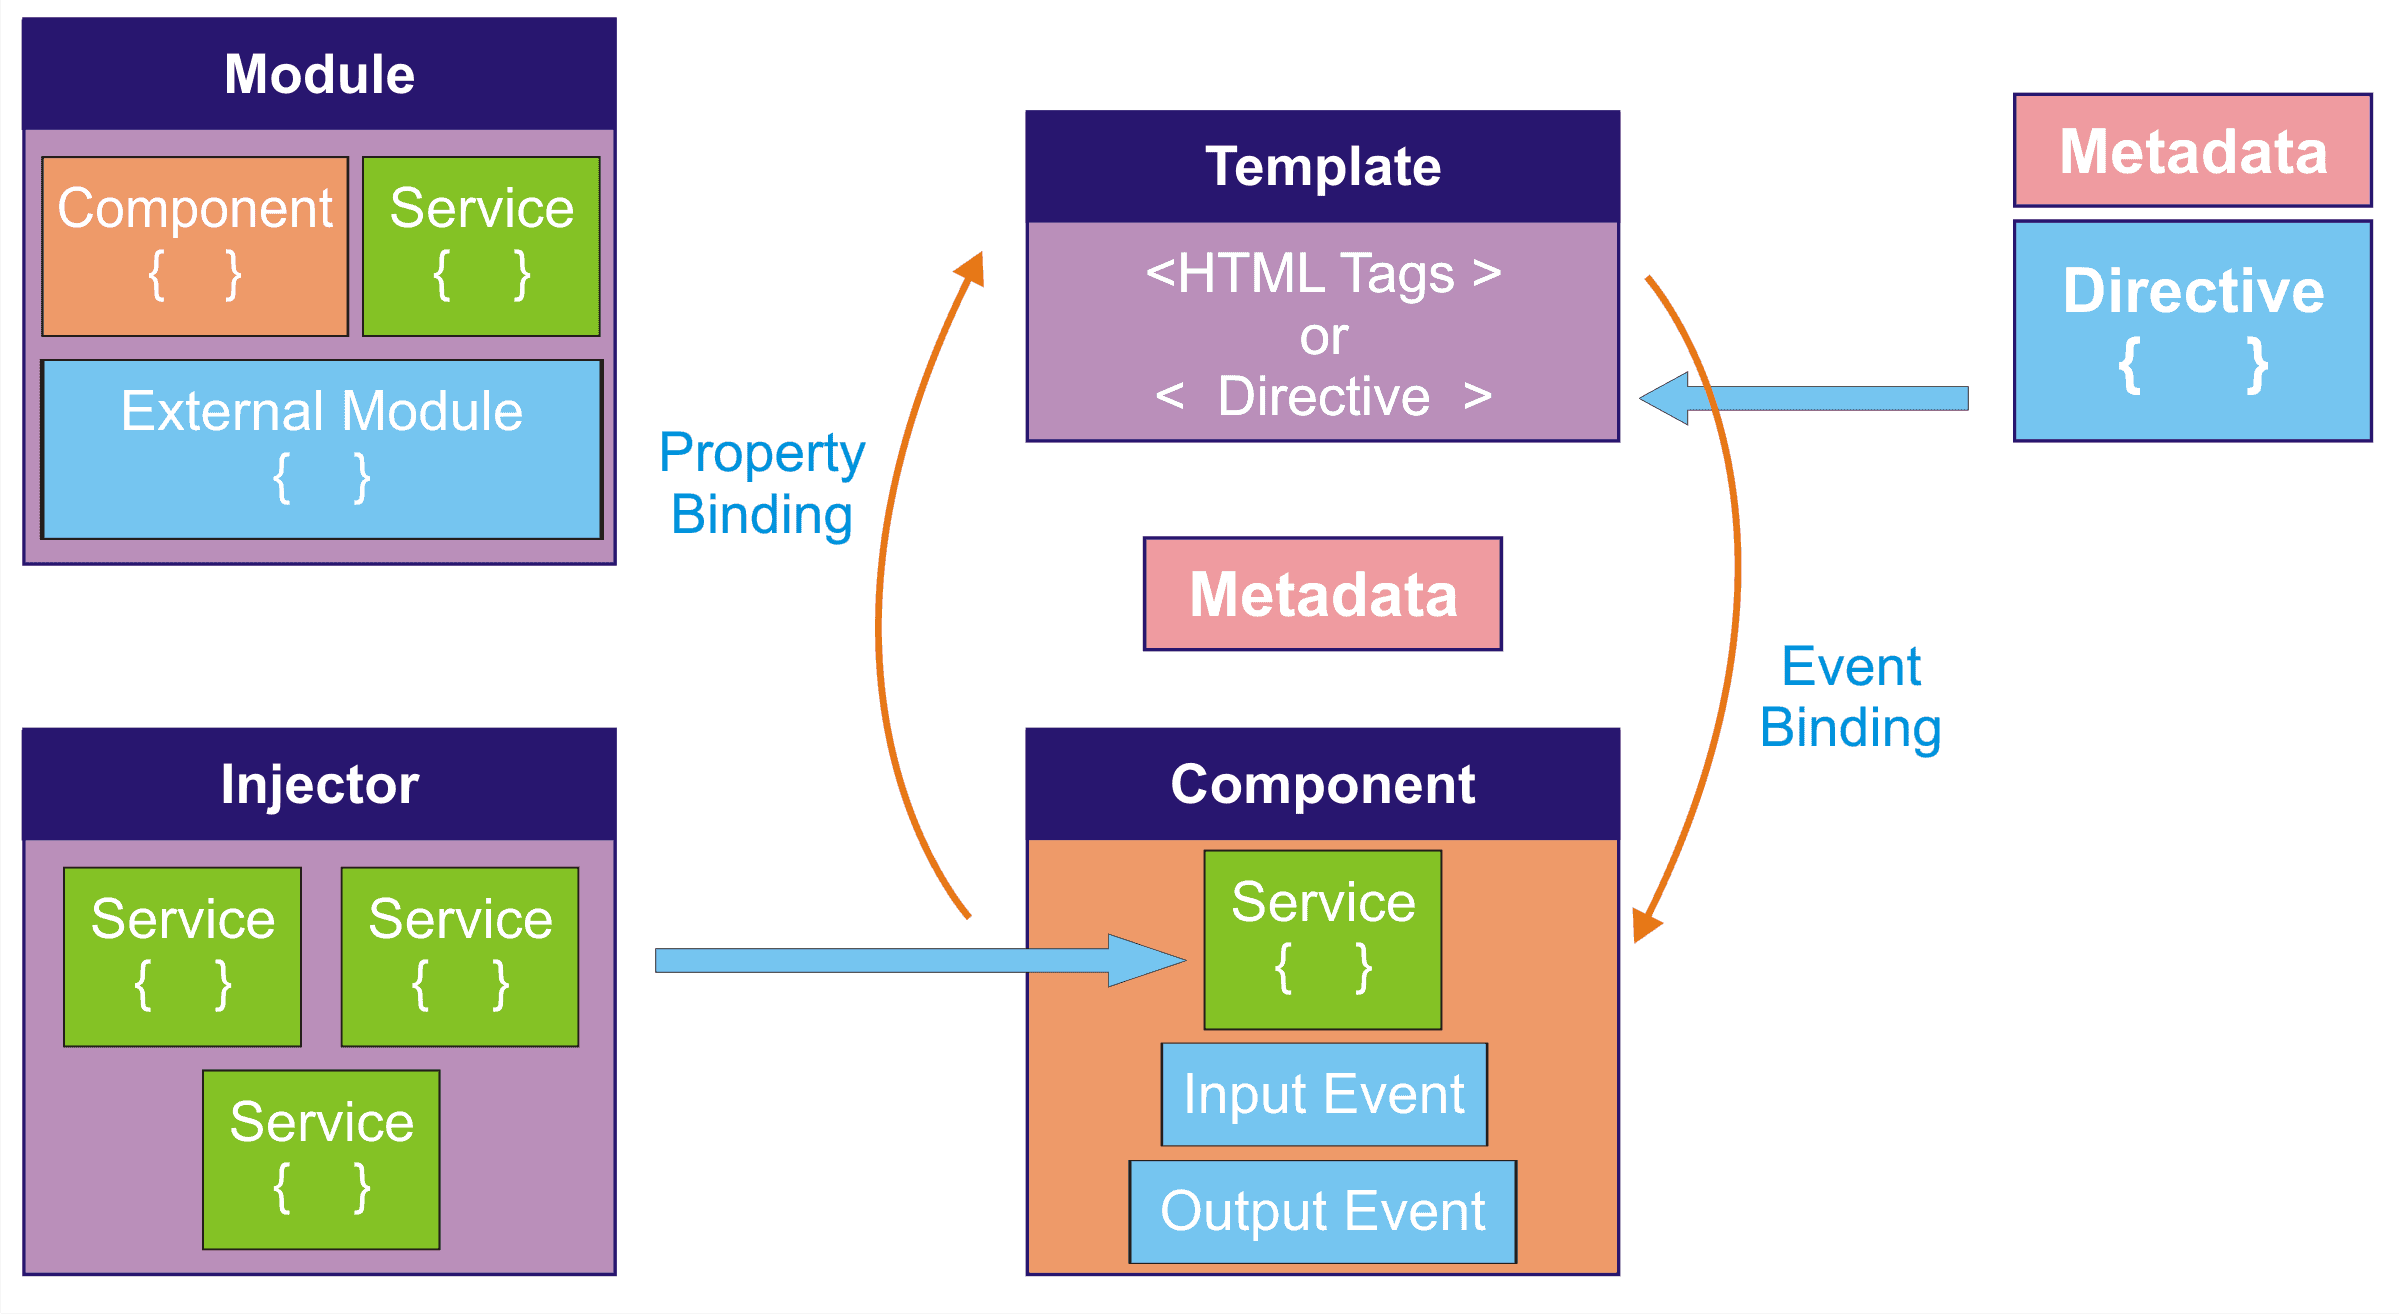
\includegraphics[width=0.8\textwidth]{Angular_Architecture.png}
	\caption{\url{https://www.ngdevelop.tech/wp-content/uploads/2017/12/Angular_Architecture.png}}
\end{figure}

\section{Spring Boot}
\begin{figure}[H]
	\centering
	
\includegraphics[width=0.3\textwidth, left]{Spring-boot-logo.jpg}
%	\caption{\url{https://dev.to/maddy/spring-boot-architecture-547i}}
\end{figure}

\section{Algoritmica}
